% Formatting
\documentclass[]{book}
\usepackage[margin = 1in, paperwidth = 6in, paperheight = 9in,twoside]{geometry}
\usepackage{microtype}
\usepackage{multicol}
\usepackage{makeidx}
\makeindex

% Graphics
\usepackage{graphicx}

% Math Packages
\usepackage{amsthm}
\newtheorem{theorem}{Theorem}[chapter]
\newtheorem{corollary}{Corollary}[theorem]
\newtheorem{lemma}[theorem]{Lemma}
% Boldface Proof
\makeatletter
\renewenvironment{proof}[1][\proofname] {\par\pushQED{\qed}\normalfont\topsep6\p@\@plus6\p@\relax\trivlist\item[\hskip\labelsep\bfseries#1\@addpunct{.}]\ignorespaces}{\popQED\endtrivlist\@endpefalse}
\makeatother

% Pseudocode Verbatim Environment
\usepackage{fancyvrb}
\renewcommand{\theFancyVerbLine}{%
 {\small\arabic{FancyVerbLine}}}  % line numbers
 \fvset{numbers=left,xleftmargin=10mm}

% Table of Contents custom package
\usepackage{tocloft}
\usepackage[nottoc]{tocbibind}
% Removes dots from ToC
\renewcommand{\cftdot}{}
% Customizes fonts for ToC; removes dots; changes style of text and indentation
\renewcommand{\cfttoctitlefont}{\LARGE\bfseries\MakeUppercase}
\renewcommand{\cftchapfont}{\Large\bfseries}
\renewcommand{\cftchappagefont}{}
\renewcommand{\cftsecpresnum}{\bfseries}
\renewcommand{\cftchapaftersnum}{.}
\renewcommand\cftchapafterpnum{\vskip 10pt}
\setlength{\cftchapnumwidth}{30pt}
\setlength{\cftsecindent}{35pt}
\setlength{\cftbeforechapskip}{15pt}
\normalsize{\settocbibname{References}}
\normalsize{\setindexname{Index}}

% Responsible for removing headings off clear pages
\makeatletter
\renewcommand*{\cleardoublepage}{\clearpage\if@twoside \ifodd\c@page\else
\hbox{}%
\thispagestyle{empty}%
\newpage%
\if@twocolumn\hbox{}\newpage\fi\fi\fi}
\makeatother

% Title page
\author{}
\title{}
\date{}

% MACROS
\newcommand{\runtime}{\textbf{Running time:}}
\newcommand{\memory}{\textbf{Memory space:}}

% hyperref must be the last command in preamble
\usepackage[pdftex]{hyperref}

\begin{document}
  \frontmatter
  \thispagestyle{empty}
  \begin{center}
    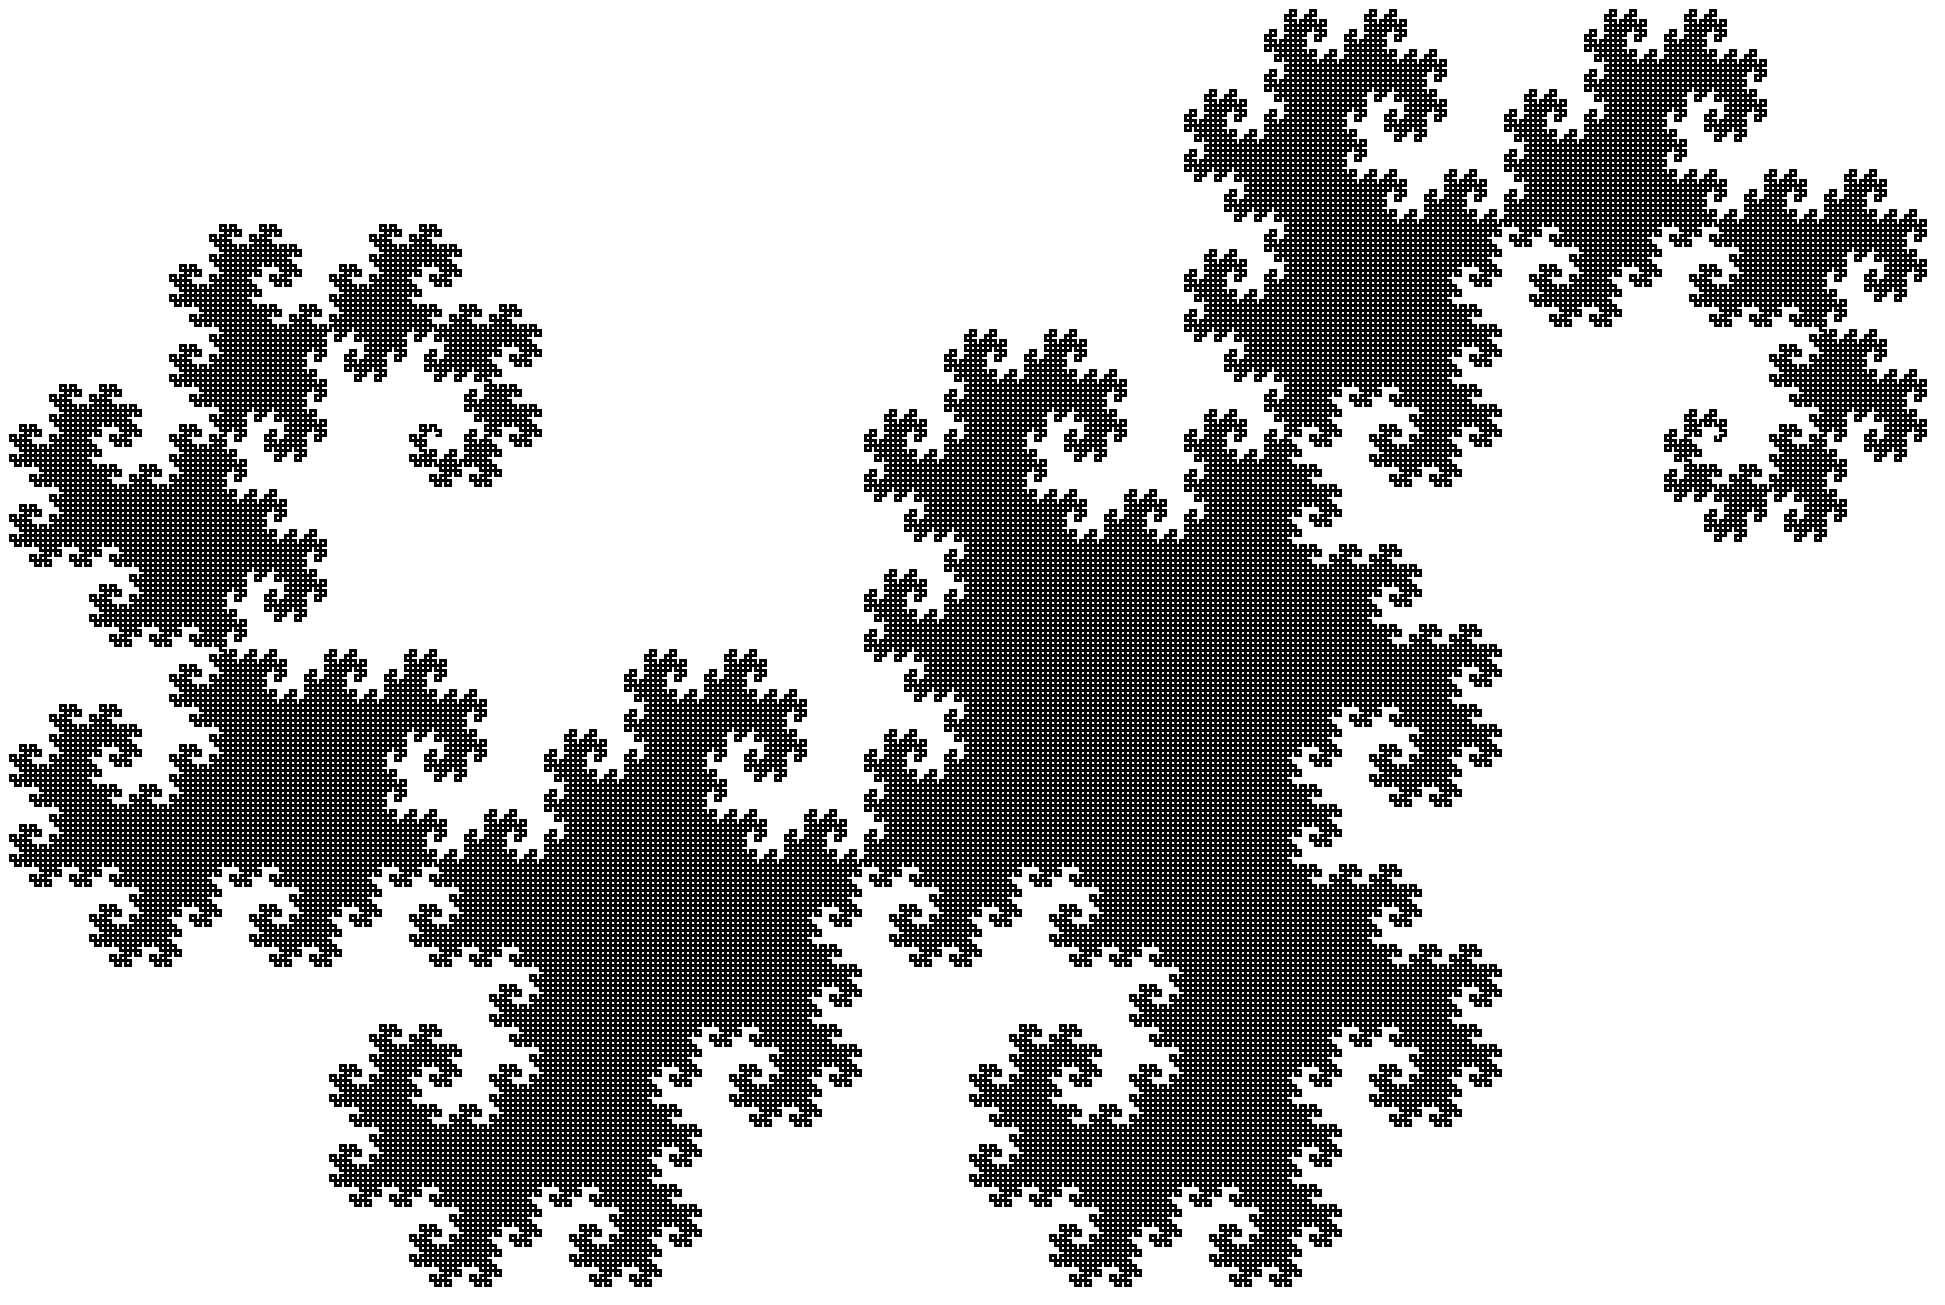
\includegraphics[scale=0.17]{dragon16.png}
  \end{center}
  \clearpage
  \newgeometry{margin = 1in, top=0.75in, paperwidth = 6in, paperheight = 9in,twoside} %customize margins for special pages
  \tableofcontents
  \thispagestyle{empty}

  \chapter*{Preface}
  \indent The goal of this book is to serve as a preparation guide for coding competitions.
  I should mention that this is a \textit{personalized} reference book for myself and my team.
  As a consequence, more attention is given over to writing for Java and C++.\\
  \indent Some competition environments allow texts with a certain criterea. ICPC\index{ICPC} World Finals
  rules that a team may bring a \textbf{Team Reference Document}, a document containing up to
  25 pages of reference materials, single-sided, letter or A4 size. This book does not
  follow the requisite, but we advise you to look at our appendix section.\\
  \indent We have included an two appendixes. Appendix 1 is devoted to common data structures we
  encountered using Java and C++. Appendix 2 includes common mathematical formulas for reference.
  \restoregeometry  %Restore to original margins

  \mainmatter
  \chapter{Behind the Big O}
  \section{Reductions}
  FILL
  \chapter{Trees}

  \chapter{Graphs}
  Graphs are a fundamental data structure in the world of programming. Formally
  a \textbf{graph}\index{graph} G consists of a finite nonempty set V of objects called \textbf{vertices}
  and a set E called \textbf{edges}. G is an ordered pair of sets V and E. $$ G = (V,E)$$
  \indent Graphs are often used to represent physical entities (a network of roads, relationship
  between people). Common graph problems include shortest paths, number of minimum cuts,
  strongly connected components \ldots.

  \section{Breadth-First Search}
  Consider you're playing an all-time classic, LoZ: Ocarina of Time. Being the
  completionist that you are, you want to open every single chest in all of the dungeons. How would
  you traverse the dungeon?\\
  \indent Often labeled as a `cautionary search', the plan of \textbf{Breadth-First Search}
  is to uniformally explore the nodes of a graph outwards. In BFS, we pick a starting node
  $n_1$ and visit all of $n_1$'s neighbors before visiting their neighbors. Using this algorithm
  allows us to visit all rooms of a dungeon without roaming too deep. \\
  \indent The main perk of BFS over other search algorithms is it can compute shortest
  paths\index{shortest path} in unweighed graphs\index{unweighed graph}.

  \section{Depth-First Search}
  If BFS is the cautious and tentative exploration strategy, then \textbf{Depth-First Search}
  \index{DFS}(DFS) is its more aggressive cousin. DFS explores aggressively, delving deeper
  into the graph and backtracks only when necessary.\\
  \indent The implementation of DFS is similar to BFS, but instead of using a queue\index{queue}, we
  use a stack\index{stack}. Another method is to use recursion\index{recursion}.\\
  \begin{Verbatim}
    void search(Node root){
      if(root == null) return;
      visit(root);
      root.visited = true;
      for each (Node n in root.adjacent) {
        if (n.visited == false) {
          search(n);
        }
      }
    }
  \end{Verbatim}
  \runtime{} $O(V+E)$\\\\
  Why use DFS over BFS? DFS has its own catalog of applications that can't be replicated
  using BFS.
  \begin{itemize}
    \item Computing a topological ordering of directed acyclic graphs\footnote{
    Note: G has a directed cycle $\Longrightarrow$ No topological ordering
    }
    \item Computing strongly connected components of directed graphs
  \end{itemize}

  \subsection*{Topological Sort}
  Khoa is really interested in artificial intelligence, so much so that before he graduates,
  he wants to take the course offered by the computer science department, CS 4242 (X).
  However, before he can enroll in CS 4242, he must have completed its prerequisites.\\
  \indent The prerequisites for CS 4242 are CS 3304 (W) and MATH 3332 (V). CS 3304 and MATH 3332
  also have a prerequisite, MATH 1190 (S).

  The sequence of which Khoa can take his classes can be arranged via topological sort.
  There are two sequences which Khoa can take.

  A \textbf{topological ordering}\index{topological ordering} of a directed graph G
  is a labeling $f$ of G's nodes such that:
  \begin{enumerate}
    \item the $f(v)$'s are the set ${1,2,\ldots, n}$
    \item $(u,v) \in G \Rightarrow f(u) < f(v)$
  \end{enumerate}

  As long as our structure is a directed acyclic graph (DAG), we can compute a topological ordering.
  Every DAG has a sink vertex. Remove the sink vertex, and the remaining graph is a DAG. (Unless
  $|v| < 1$) The pseudocode for a topological sort is as follows:
  \begin{Verbatim}
    DFS(graph G, start vertex s) {
      visit(s);
      for each edge (s,v) {
        if(v.visited == false)
          DFS(G, v);
      }
      set f(s) = current_label
      current_label--;
    }

    topologic_sort(graph G) {
      mark all nodes unexplored;
      current_label = n;
      for each vertex $v \in G$ {
        if(v.visited == false)
          DFS(G, v);
      }
    }
  \end{Verbatim}
  \runtime{} $O(V+E)$\\
  \memory{} $O(V+E)$
  \begin{proof}
    Take any edge, $(u,v)$. We will show that $f(u) < f(v)$.\\\\
    \indent Case 1: u is visited by DFS before v\\
    u will recursively call v, which will continue DFS. Eventually v will exhaust
    its adjacent neighbors and become a sink vertex before u. $f(u) < f(v)$\\\\
    \indent Case 2: v is visited by DFS before u\\
    v makes recursive DFS calls. u will never be visited during these recursively calls,
    otherwise the graph would contain a directed cycle. As a result, v will become a sink
    vertex before u is visited. $f(u) < f(v)$
  \end{proof}

  \subsection*{Strongly Connected Components}
  The \textbf{strongly connected components}\index{SCC} of a directed graph G are defined
  as the equivalence classes of the relation $u\sim v \Leftrightarrow \exists$ path$(u,v)$ and
  path$(v,u)$. SCCs can be computed using \textbf{Kosaraju's Two Pass algorithm}
  \index{Kosaraju}.

  Kosaraju's Two Pass Algorithm
  \newtheorem{Kosaraju}{Theorem}[section]
  \begin{Kosaraju}
    Can compute SCC in $O(m+n)$
  \end{Kosaraju}
  \chapter{Weighted Graphs}

  \backmatter
  \setlength{\cftbeforechapskip}{15pt}
  \renewcommand\cftchapafterpnum{\vskip 10pt}
  \renewcommand\bibname{\large{References}}
  \newgeometry{margin = 1in, top=0.25in, paperwidth = 6in, paperheight = 9in,twoside}
  \begin{thebibliography}{9}
  \bibitem{latexcompanion}
  Michel Goossens, Frank Mittelbach, and Alexander Samarin.
  \textit{The \LaTeX\ Companion}.
  Addison-Wesley, Reading, Massachusetts, 1993.

  \bibitem{einstein}
  Albert Einstein.
  \textit{Zur Elektrodynamik bewegter K{\"o}rper}. (German)
  [\textit{On the electrodynamics of moving bodies}].
  Annalen der Physik, 322(10):891–921, 1905.

  \bibitem{knuthwebsite}
  Knuth: Computers and Typesetting,
  \\\texttt{http://www-cs-faculty.stanford.edu/\~{}uno/abcde.html}
  \end{thebibliography}

  \appendix
  \chapter{\large{Appendix I: \textnormal{Data Structures}}}
  \chapter{\large{Appendix II: \textnormal{Mathematical Formulae}}}
  \printindex
\end{document}
